\documentclass{report} 
\usepackage{pdfsync}
\usepackage{epsfig} 
\usepackage{amsfonts}  
\usepackage{fullpage}
% \usepackage{underscore}

\begin{document}

\title{Random Realizations: Gaussian process classes for Python\\
Algorithm documentation}
\author{Anand Patil}
\maketitle
\tableofcontents
    
\chapter{Introduction}\label{cha:introduction} % (fold)

This document describes the algorithms under the Random Realizations package, a handful of Python building blocks designed to make unrestricted and innovative use of GPs more accessible. These building blocks are:
\begin{itemize}
    \item Objects representing mean functions, covariance functions, and realizations of Gaussian processes.
    \item A function that implements standard Gaussian process regression by `imposing' normally-distributed observations on the mean and covariance functions.
    \item An object representing GP realization-valued random variables.
    \item Infrastructure for incorporating such random variables into a general-purpose Markov Chain Monte Carlo (MCMC) \cite{gelman} package along the lines of Bugs \linebreak (\texttt{www.mrc-bsu.cam.ac.uk/bugs/}).
\end{itemize}
Random Realizations attempts to provide an intuitive implementation by relying on objects that closely resemble the functional concepts they represent. It allows users to specify and fit probability models of their own devising involving Gaussian processes based on a conceptual understanding, without worrying about the underlying linear algebra.

The source code and a user guide are available from 
\begin{verbatim}
    code.google.com/p/gaussian-process.
\end{verbatim}

The MCMC package with which Random Realizations interfaces is PyMC, version 2.0 and higher (\texttt{code.google.com/p/pymc}). PyMC is an open-source collaboration between Christopher Fonnesbeck, David Huard and myself. Like Random Realizations, it is implemented in Python.


\section{Terminology, notation and calling conventions} 

In this document, the building blocks' user interfaces are presented Python, but their internal workings and the algorithms they use are presented in pseudocode. An overview of the notation and some terminology from object-oriented programming follows.

\begin{itemize}
    \item A \emph{class} is a prototype for a class of objects, each of which is an \emph{instance} of the class. New class instances are created by passing initialization arguments to the class. For example, a new instance of class \texttt{Realization} called $f$ would be created from mean function $M$ and covariance function $C$ as follows:
\begin{verbatim}
    f = Realization(M, C).
\end{verbatim}
    
    \item An \emph{attribute} of an object is an item associated with the object, which can be accessed via the object. I will denote object attribute access with a period. If $G$ is a random variable valued as a Gaussian process realization, \texttt{G.value} gives access to its current value (which is an instance of class \texttt{Realization}, like \texttt{f}).
    
    \item A \emph{method} of an object is a special attribute of the object that can be called like a function. Calling an object's method causes the object to do something. If $C$ is a covariance function, The call \texttt{C.cholesky(x)} causes $C$ to compute the Cholesky factorization of its evaluation on the vector $x$ and return it.

    \item A \emph{callable object} is an object that can be called like a function. For example, the Gaussian process realization objects are callable because they are intended to represent random functions:
\begin{verbatim}
    f(x)
\end{verbatim}
would evaluate $f$ at vector of values $x$.% Realizations need to `remember' all previous calls, so they cannot be represented by simple functions (at least not in Python).
\end{itemize}

Note that there is much more to object-oriented programming than this, and that different authors have varying views on the fundamental concepts. See Armstrong \cite{OOP_review} for a review of object-oriented concepts in practice or Silvert \cite{silvert_OOP} for an introduction to object-oriented programming in the context of ecological simulation. 

\medskip
Code is represented in a typewriter font: 
\begin{verbatim}
    f = Realization(M, C)
\end{verbatim}
Square brackets denote array indexing, and colons indicate ranges of consecutive integers:
\begin{eqnarray*}
    K[1:m,2:n] = \left[\begin{array}{ccc}
    K[1,2]&\cdots&K[1,n]\\
    \vdots&\ddots&\vdots\\
    K[m,2]&\cdots&K[m,n]
    \end{array}\right].
\end{eqnarray*}
Array indexing begins at $1$ (note that in numerical Python indexing begins at 0). Curly braces denote concatenation:
\begin{eqnarray}
    \{x,y\} = [x[1]\ldots x[n_x], y[1]\ldots y[n_y]].
\end{eqnarray}

Specialized notation is used for evaluating functions on vector arguments. Here $\mathbf x$ is a vector of values and $x$ is a single value. For one-place functions (mean functions and realizations),
\begin{eqnarray}
    f(\mathbf x) = [f(x[1])&\ldots&f(x[n])].
\end{eqnarray}
For two-place functions (covariance functions),
\begin{equation}
    \begin{array}{lll}
        C(x[1], x) &=& \left[
        \begin{array}{ccc}
            C(x[1], x[1]) & \cdots & C(x[1], x[n])
        \end{array}
        \right],\\
        C( x, x) & = &\left[
        \begin{array}{ccc}
            C( x[1], x[1]) & \cdots & C( x[1], x[n]) \\\vdots & \ddots & \vdots \\C( x[n], x[1]) & \cdots & C( x[n], x[n])
        \end{array}
        \right],\\
        C( x,x[1]) & = &\left[
        \begin{array}{ccc}
            C(x[1],x[1]) &\cdots& C(x[n],x[1])
        \end{array}
        \right]^T.
    \end{array}
\end{equation}

\chapter{The basic objects and normally-distributed observations}\label{cha:basics} % (fold)
\section{Mean functions}

Objects of class \texttt{Mean} represent mean functions. These objects are `wrappers' for ordinary functions, meaning that their purpose is to mediate between the ordinary functions and the outside world. A mean function $M$ can be created from an ordinary Python function $g$ as follows:
\begin{verbatim}
    def g(x, a, b, c):
        return a * x ** 2 + b * x + c
    
    M = Mean(g, a = 2, b = 1, c = 3).
\end{verbatim}
The first initialization argument is the function $g$, and the subsequent initialization arguments are values for the extra parameters that $g$ requires. These values are `memorized' by $M$ and passed to $g$ at each subsequent call, so the call
\begin{verbatim}
    M(5)
\end{verbatim}
is equivalent to
\begin{verbatim}
    g(5, 2, 1, 3).
\end{verbatim}
Mean's only notable attribute is a method called \texttt{observe}, which will be described in chapter \ref{sec:obs} 

\section{Covariance functions} \label{sec:cov} 

GP covariance functions are represented by the class \texttt{Covariance}, and like \texttt{Mean} instances they are wrappers for ordinary functions. However, the underlying functions of \texttt{Covariance} instances take two input arguments. A Gaussian covariance function could be produced as follows:
\begin{verbatim}
    def euclidean_distance(x, y):
        D = matrix((len(x), len(y)))
        for i in range(len(x)):
            for j in range(len(y)):
                D[i,j] = sqrt((x[i] - y[j]) ** 2)
        return D
    
    def gaussian(x, y, amp, scale):
        C = euclidean_distance(x, y)
        C *= scale
        for i in range(len(x)):
            for j in range(len(y)):
                C[i,j] = amp * exp(- (C[i,j] / scale) ** 2)
        return C
        
    C = Covariance(gaussian, amp = 10, scale = .1)
\end{verbatim}
The separation between the two stages of computation of the covariance matrix,
\begin{enumerate}
    \item computation of a distance matrix
    \item overwriting the distance matrix with an isotropic and stationary covariance function,
\end{enumerate}
is emphasized intentionally. This arrangement makes it relatively painless to accomodate new coordinate systems and to build in anisotropy and/or nonstationarity by deforming the input space \cite{sampson} or by redefining distance \cite{pachische}. Conversely, new functional forms can be easily applied to all available coordinate systems. Random Realizations' `plugs' for such extensions are described in more detail in the documentation \cite{me_SR}.


Like \texttt{Mean} instances, \texttt{Covariance} instances memorize the extra arguments required by their underlying functions. The following two calls are equivalent:
\begin{verbatim}
    C(2, 3)
    gaussian(2, 3, 10, .1).
\end{verbatim}
Covariances can also be called with a single argument. For a vector \texttt{x}, the call
\begin{verbatim}
   C(x)
\end{verbatim}
returns a result equivalent to
\begin{verbatim}
    diag(C(x,x))
\end{verbatim}
but does not compute the off-diagonal terms.

Covariance objects have a method called \texttt{observe} that, like \texttt{Mean.observe}, will be described in \ref{sec:obs}. They have two additional methods: \texttt{cholesky} and \texttt{continue\_cholesky}.

\subsection{Covariances' Cholesky method}
The following method call with length-$n$ vectors $x$ and $V$
\begin{verbatim}
    C.cholesky(x, V)    
\end{verbatim}
returns the following items:
\begin{itemize}
    \item A length-$n$ vector of pivot indices $p$.
    \item An $m$-by-$n$ upper triangular matrix $U$ such that $U_*^TU_* = C(x,x) + \textup{diag}(V)$ for the pivoted matrix $U_* = U[1:m,q]$, where $m\le n$ and $p[q]=1:n$.
\end{itemize}
$U$ is an incomplete Cholesky factor \cite{incompchol} for $C(x,x)+\textup{diag}(V)$, with diagonal pivoting applied. If $C(x,x)+\textup{diag}(V)$ is full-rank, $m=n$ and $U$ is simply a pivoted Cholesky factor. The following algorithm, based on the algorithm implemented in the MATLAB package `chol\_incomplete' \linebreak
(\texttt{http://www.kyb.tuebingen.mpg.de/bs/people/seeger/software.html}), allows $U$ to be computed in $O(m^2n)$ operations plus a storage cost of $O(n^2)$:
\begin{itemize}
    \item $d = C(x,x)+\textup{diag}(V)$ (the diagonal can be computed without computing the full matrix)
    \item $d_* = \max d$
    \item $p=1:n$
    \item $U=$ zero matrix of size $n$ by $n$
    \item for $i$ from 1 to $n$:
    \begin{itemize}
        \item $l=$ value of index $j\in i:n$ where $d[j]$ is largest.
        \item if $d[l] / d_*<\epsilon$:
        \begin{itemize}
            \item return $p$, $U[1:i, 1:n]$. Rank of $C(x,x) + \textup{diag}(V)$ is $i$.
        \end{itemize}
        \item $d[i] \leftrightarrow d[l]$, $p[i] \leftrightarrow p[l]$, $x[i] \leftrightarrow x[l]$, $U[1:i,i] \leftrightarrow U[1:i,n]$
        \item $U[i,i]=\sqrt {d[i]}$
        \item $r$ = $C(x[i], x[i+1:n])$
        \item if $i>1$:
        \begin{itemize}
            \item $r=r-U[1:i,i]^T U[1:i,i+1:n]$
        \end{itemize}
        \item $U[i,i+1:n] = r / U[i,i]$
        \item for $j$ from $i+1$ to n:
        \begin{itemize}
            \item $d[j] = d[j] - U[i,j]^2$
        \end{itemize}
    \end{itemize}
    \item return $p$, $U[1:n, 1:n]$. $C(x,x) + \textup{diag}(V)$ is full-rank.
\end{itemize}
Similar algorithms are given by Golub and van Loan \cite{golub} and implemented in LINPACK (as subroutine \texttt{DCHDC}) \cite{Linpack}. Note that the full matrix $C(x,x)$ does not need to be computed ahead of time, and in fact if $m<n$ many of its elements will never be computed at all. More sophisticated pivot selection schemes than the greedy algorithm presented here are available, see for instance Bach and Jordan \cite{predictivechol}. 

\medskip
After iteration $i$, the diagonals $d[i+1:n]$ give the conditional variance of a realization with covariance $C$ evaluated at $x[i+1:n]$ given the value of the realization evaluated at $x[1:i]$, observed with error variance diag$(V)$. The algorithm proceeds by selecting points in order of variance conditional on points already used, and terminates when all remaining points have conditional variance less than $d_*\epsilon$.

This Cholesky factor should eventually be computed as a low-rank update \cite{Seeger} of the (diagonal) Cholesky factor of $\textup{diag}(V)$ (Matthias Seeger, pers. comm.), but I have not implemented that optimization.

\subsection{Covariances' Cholesky continuation method}
It is frequently desirable to compute an incomplete Cholesky factor for the covariance matrix
$C(\{x,y\},\{x,y\}) + \textup{diag}(\{V_x,V_y\})$ when the corresponding factor $U_x$ of $C(x,x) + \textup{diag}(V_x)$ is known. 

In this chapter, $U_x$, $p_x$ and $m_x$ denote the incomplete Cholesky factor of $C(x,x)+\textup{diag}(V_x)$ and the associated pivots and rank; $n_x$ and $n_y$ denote the lengths of $x$ and $y$. The combined length of $x$ and $y$ is denoted $n$.

The call
\begin{verbatim}
    C.continue_cholesky(x,y,Vx,Vy,Ux,px)
\end{verbatim}
efficiently computes and returns the following:
\begin{itemize}
    \item A length-$n$ vector of pivot indices $p$, $n$ being the length of $\{x,y\}$.
    \item An $m$-by-$n$ ($m\le n$) upper triangular matrix $U$ such that $U_*^TU_* = C(\{x,y\},\{x,y\}) + \textup{diag}(\{V_x,V_y\})$ for the pivoted matrix $U_* = U[1:m,q]$, where $p[q]=1:n$.
\end{itemize}

The algorithm begins as follows:
\begin{itemize}
    \item $U=$ zero matrix of size $m_x+n_y$ by $n$
    \item$U[1:m,1:n]=$ \begin{eqnarray*}
        \left\{\begin{array}{ccc}
            U_x[1:m_x,1:m_x],&U_x[1:m_x,1:m_x]^{-T} C(x[p[1:m_x]], y),&U_x[1:m_x,m_x+1:n_x]
        \end{array}\right\}
    \end{eqnarray*}
    \item $p=\{p_x[1:m_x],\ m_x+1:m_x+n_y,\ p_x[m_x+1:n_x]\}$
    \item $x=\{x[p_x[1:m_x]],\ y,\ x[p_x[m_x+1:n_x]]\}$.
\end{itemize}

The initial layout of $U$ looks like it would during the call
\begin{verbatim}
    C.cholesky({x, y}, {Vx, Vy})
\end{verbatim}
when $i=m_x$, so the rest of the algorithm is the same as the incomplete Cholesky algorithm above, but with $i$ ranging from $m_x+1$ to $n$. The expense of this algorithm is $O(n(m^2-m_x^2))+O(m_x^2 n_y)$, plus a storage cost of $O(n(m_x+n_y))$.

\subsection{Basis covariances}\label{sec:basis}

In some cases, significant speed gains can be realized by representing a Gaussian process as a linear combination of a finite set of basis functions $e_i$ with normally-distributed coefficients $c_i$:
\begin{eqnarray*}
    \left.
    \begin{array}{ll}
        f(x) = M(x) + \sum_{i_0=0}^{n_0-1}\ldots \sum_{i_{N-1}=0}^{n_{N-1}-1} c_{i_1\ldots i_{N-1}} e_{i_1\ldots i_{N-1}}(x), &
        \{c\}\sim \textup{N}(0,K). 
    \end{array}
    \right\}
    \Rightarrow f \sim \textup{GP}(M,C) 
\end{eqnarray*}
where the covariance function $C$ is defined by
\begin{eqnarray*}
    C(x,y)=\sum_{i_0=0}^{n_0-1}\ldots \sum_{i_{N-1}=0}^{n_{N-1}-1} \sum_{j_0=0}^{n_0-1}\ldots \sum_{j_{N-1}=0}^{n_{N-1}-1} e_{i_0\ldots i_{N-1}}(x) e_{j_1\ldots j_{N-1}}(x) K_{i_0\ldots i_{N-1}, j_1\ldots j_{N-1}}.
\end{eqnarray*}

Particularly successful applications of this idea are:
\begin{description}
    \item[Random Fourier series:] $e_i(x) = \sin(i\pi x/L)$ or $\cos(i\pi x/L)$, for instance \cite{spanos}.
    \item[Gaussian process convolutions:] $e_i(x) = \exp(-(x-\mu_i)^2)$, for instance \cite{convolution}.
    \item[Splines:] Several spline interpolations can be represented as linear combinations of basis functions, usually polynomials. \cite{micula, lang_pspline} 
\end{description}

Such covariances are represented by the classes \texttt{BasisCovariance} and \texttt{SeparableBasisCovariance}, which have the same methods and behavior as \texttt{Covariance}. The first initialization argument to these objects are bases, which are lists or arrays of functions. More details are given in the user guide.

\texttt{BasisCovariance}'s Cholesky and Cholesky continuation methods are essentially the same as those of \texttt{Covariance}, but only a $\min (N,n)$-by-$n$ matrix is allocated ahead of time for the Cholesky factors where $N$ is the total number of elements in $c$. The diagonal and row vectors are computed on demand in the obvious way.

\section{Normally-distributed observations}\label{sec:obs}

The \texttt{observe} function and the \texttt{observe} methods of \texttt{Mean} and \texttt{Covariance} share responsibility for solving the following conjugate statistical model:
\begin{equation}
    \label{regprior}
    \left.\begin{array}{l}
        D_i \stackrel{\tiny{\textup{ind}}}{\sim} \textup{N}(f(o_i), V_i)\\
        f \sim \textup{GP}(M,C)\\
    \end{array}\right\}\Rightarrow f|D \sim \textup{GP}(M_o, C_o).
\end{equation}
More specifically, the call 
\begin{verbatim}
    observe(M, C, o, D, V)
\end{verbatim}
essentially transforms $M$ and $C$ to $M_o$ and $C_o$ above by calling the \texttt{observe} methods.

The formulas for $M_o$ and $C_o$ are as follows, for arbitrary input vectors $x$ and $y$:
\begin{eqnarray*}
    M_o(x) = M(x) + C(x,o)[C(o,o) + \textup{diag}(V)]^{-1}(D-M(o))\\
    C_o(x,y) = C(x,y) - C(x,o)[C(o,o) + \textup{diag}(V)]^{-1}C(o,y).
\end{eqnarray*}
The ultimate effect of the call to \texttt{observe} is the following:
\begin{itemize}
    \item to store a square rank-$m_o$ Cholesky factor $U_o[1:m_o,1:m_o]$ and associated pivot vector $p_o$ of $C(o[p_o[1:m_o]],o[p_o[1:m_o]]) + \textup{diag}(V[p_o[1:m_o]])$ in \texttt{C}
    \item to store the vector $U_o[1:m_o,1:m_o]^{-T}(D[p_o[1:m_o]] - M(o[p_o[1:m_o]]))$ in \texttt{M}.
\end{itemize}
This information can be used to compute the above formulas efficiently when input vectors $x$ and $y$ are provided.

Denote $o[p_o[1:m_o]]$ by $o_*$, the complement $o[p_o[m_o+1:n_o]]$ by $o_{**}$, and define $V_*$, $V_{**}$, $D_*$ and $D_{**}$ analogously. As discussed earlier, due to the properties of the incomplete Cholesky decomposition the conditional variance of $f(o_{**})|D_*$ is less than or equal to $\epsilon$ times the maximum unconditional variance $d_*$ of $f(o_*)$.

\bigskip
Normally-distributed observations are used in three important ways:
\begin{itemize}
    \item Simple nonparametric regression: direct user application of model (\ref{regprior}).
    \item Gibbs sampling a Gaussian process realization when its Markov blanket \cite{jensen}  is of the form (\ref{regprior}).
    \item After each call, a \texttt{Realization} object `remembers' the values it returned by means of the \texttt{observe} methods (with $V=0$) to maintain consistency.
\end{itemize}

Covariances' and means' observe methods are fairly complicated, but most users should not need to call them directly. Denote by $o_p$, $D_p$ and $V_p$ the values at which observations have been made previously, the observed values and the corresponding variances. These vectors may be length-0. Denote by $o_n$, $D_n$ and $V_n$ the analogous vectors corresponding to new observations, and by $o$, $D$ and $V$ the concatenation of these. Denote by $n_p$ and $m_p$ the size and rank of $C(o_p,o_p)$, and by $n$ and $m$ the rank of $C(\{o_p,o_n\},\{o_p,o_n\})$. 

\subsection{Covariances' observe methods}
The call
\begin{verbatim}
    C.observe(o, V)
\end{verbatim}
does the following:
\begin{itemize}
    \item Endows \texttt{C} with the following attributes:
    \begin{itemize}
        \item An incomplete rank-$m$ Cholesky factor $U_o$ of $C(\{o_p,o_n\},\{o_p,o_n\}) + \textup{diag}(\{V_p,V_n\})$, truncated to be square.
        \item A corresponding vector $p$ of pivots.
    \end{itemize}
    \item Returns the following values:
    \begin{itemize}
        \item The subvector $o_*=o[p[1:m]]$ that is represented in the rows of $U_o$.
        \item $I_*=p[1:m]$
        \item A matrix $U_{o_n|o_p}$ such that $U_{o_n|o_p}^TU_{o_n|o_p} = C_{o_p}(o_n,o_n)$ up to order $\epsilon$. This matrix is given by
        \begin{eqnarray*}
            U_{o_n|o_p} = U_o[m_p+1 : m,q[m_p+1: n]],
        \end{eqnarray*}
        where $p[q] = 1:n$.
    \end{itemize}
\end{itemize}

After a covariance's observe method has been called, calls to the covariance will return values according to $C_o$ rather than $C$ in equation (\ref{regprior}). The return values $o_*$ and $I_*$ are used to prepare input values for \texttt{Mean.observe}, and the return value $U_{o_n|o_p}$ is used by realizations to generate new values.

\subsection{Basis covariances' observe methods}
Unfortunately, in order for basis covariances' computational advantages to be fully exploited their observe methods need to work differently. The model
\begin{eqnarray*}
    D_i \stackrel{\tiny{\textup{ind}}}{\sim} \textup{N}(f(o_i, V_i))\\
    f = M + \sum_{i=1}^N c_i e_i(o)\\
    c \sim \textup{N}(0, K) 
\end{eqnarray*}
can be solved to obtain the following heirarchical posterior for $f$:
\begin{eqnarray*}
    f = M_o + \sum_{i=1}^N c_i e_i(o),\\
    c|D \sim \textup{N}(0, K_o) 
\end{eqnarray*}
where
\begin{eqnarray*}
    K_o = K - KE(o)(E(o)^TKE(o) + \textup{diag}(V))^{-1}E(o)^TK,\\
    M_o(x) = M(x) + E(x)^TKE(o)(E(o)^TKE(o) + \textup{diag}(V))^{-1}(D-M(o))
\end{eqnarray*}
where $E(o)$ is the matrix obtained by stacking the evaluations of the basis functions. When observed, basis covariances simply store a Cholesky factor of $K_o$.

\bigskip
When a basis covariance's observe method is called with new observations $o_n, D_n, V_n$ and previous observations $o_p, D_p, V_p$, the following happen:
\begin{itemize}
    \item The basis covariance is endowed with the following attributes:
    \begin{itemize}
        \item An incomplete Cholesky factor  $Q_{\{o_p,o_n\}}$ of $K_{\{o_p,o_n\}}$.
        \item A corresponding vector $q$ of pivots.
        \item A rank-$m$ incomplete Cholesky factor $U_o$ of $C(\{o_p, o_n\}, \{o_p, o_n\}) + \textup{diag}(\{V_p, V_n\})$, truncated to be square.
        \item A corresponding vector $p$ of pivots.
    \end{itemize}
    \item The following are returned:
    \begin{itemize}
        \item The subvector $o_*$ of $o$ represented in the rows of $U_o$
        \item The corresponding index vector $I_*$, so that $o[{I_*}] = o_*$.
    \end{itemize}
\end{itemize}
Basis covariances do not return the matrix $U_{o_n|o_p}$, because realizations drawn from basis covariances do not need this to produce new values.

\subsection{Means' observe methods}
Means' observe methods are called as follows:
\begin{verbatim}
    M.observe(C, o*, d*)
\end{verbatim}
where $o_*=o[{I_*}]$ and $d_*=d[{I_*}]$. After a mean's observe method is called, calls to the mean will return values from $M_{\{o_p, o_n\}}$ rather than $M_{o_p}$.

A call to a mean's observe method endows the mean with the following attributes:
\begin{itemize}
        \item References to $U_o$ and $\{o_p, o_n\}$, taken from $C$.
        \item The vector $U_o^{-T} (D[I_*] - M(o[I_*]))$. This vector is computed efficiently from $U_o[1:m_p,1:m_p]^{-T} (D[p[1:m_p]] - M(o[p[1:m_p]]))$ if previous observations have been made.
\end{itemize}

If $C$ is a basis covariance, the call endows the mean with different attributes:
\begin{itemize}
    \item References to $U_o$ and $[o_p, o_n]$, taken from $C$.
    \item The vector $KE(o)(E(o)^TKE(o) + \textup{diag}(V))^{-1}(f(o)-M(o))$, computed efficiently.
\end{itemize}

Means' observe methods do not return any values.

\subsection{The observe function}
The call \texttt{observe(M, C, o, D, V)} presented above simply does the following:
\begin{itemize}
    \item Calls \texttt{C}'s observe method with $o$ and $V$.
    \item Calls \texttt{M}'s observe method using the output of the previous call, plus $D$.
    \item Optionally calls \texttt{cross\_validate} (see below), and raises an error if the return value is false.
\end{itemize}

\subsection{Cross-validation}
The incomplete Cholesky decomposition provides numerical stability; even if the covariance matrix is singular, calls to \texttt{observe} will execute successfully. However, because the incomplete Cholesky decomposition effectively ignores certain datapoints it is sometimes desirable to check those datapoints for consistency post hoc. 

The function \texttt{predictive\_check} optionally checks the remaining data values $D_{**}$ against $M_{o_*}(o_{**})$, and raises an error if any elements disagree by more than ten upper-bound standard deviations $\sqrt{\epsilon d_*}$, where $\epsilon$ can be set using the \texttt{relative\_precision} parameter in \texttt{Covariance}'s init method.

\section{Gaussian process realizations}

Gaussian process realizations are represented by callable objects of class \texttt{Realization}, whose initialization arguments are a mean function and a covariance function:
\begin{verbatim}
    f = Realization(M, C).
\end{verbatim}
Realizations can also be forced to take values $y$ on input values $m$:
\begin{verbatim}
    f = Realization(M, C, y, m).
\end{verbatim}
This is useful for Metropolis algorithms. If a realization is created this way, the initial values $y$ are checked for consistency using the cross-validation scheme described above at initialization.

Gaussian processes are usually considered probability distributions for functions, and since realizations are draws from such distributions they behave like functions once they are created. The call \texttt{f(x)} returns values just like the call \texttt{cos(x)}.

\bigskip
In order to provide this appealing behavior, realizations create internal copies of their mean and covariance functions upon creation. Denote by $x$ the concatenation of all unique values at which $f$ has been evaluated already ($x$ initially has length 0), and by $f_x$ the corresponding return values. The return value for the call \texttt{f(y)} is generated as follows:
\begin{itemize}
    \item $x$ is searched for elements of $y$. If any are found, the corresponding return values are recorded. Denote by $y_*$ the elements of $y$ that are not in $x$.
    \item The internal covariance's \texttt{observe} method is called with mesh $y_*$ and variance 0.
    \item The internal mean is evaluated at $y_*$.
    \item Recall that the third return value of \texttt{Covariance.observe}, $U_{o_n|o_p}$, gives the Cholesky factor of the covariance of $f(y_*)|f(x)$. This Cholesky factor is used to generate values for $f(y_*)$.
    \item The internal mean's \texttt{observe} method is called with mesh $y_*$, values $f(y_*)$, and the internal covariance.
    \item The values $f(y_*)$ are returned.
\end{itemize}

Note that even if the Cholesky factor is low-rank, no cross-validation is necessary because any nearly-determined values of $f(y_*)$ are known a priori to fall close to their mean.

\subsection{GP realizations with basis covariances} 
Calls to GP realizations will get slower as the length of $o_p$ increases. One of the most appealing features of the \texttt{BasisCovariance} class is that it prevents this degradation from happening. However, the tradeoff is that the expense of calls tends to increase exponentially with spatial dimension.

If a realization is initialized with a \texttt{BasisCovariance} instance, it draws values for its coefficients immediately (the covariance matrix of the coefficients is factorized using an incomplete Cholesky decomposition in case it happens to be low-rank). Return values for subsequent calls to the realization are computed by simply evaluating the mean function and basis functions. Arguments are not checked for repeat calls.

\chapter{Incorporating Gaussian processes in larger probability models}\label{sec:PyMC} 

Random Realizations includes objects that allow Gaussian processes to be mixed into probability models involving more mundane random variables specified using the open-source Markov Chain Monte Carlo package PyMC (\texttt{code.google.com/p/pymc}). PyMC is implemented in Python like Random Realizations, and has a decentralized approach to model-fitting that is designed to encourage such extensions.

This chapter begins with a brief desccription of the basic building blocks of PyMC. These are:
\begin{itemize}
    \item The \texttt{Stochastic} class, representing random variables (stochastic nodes in WinBugs).
    \item The \texttt{Deterministic} class, representing variables whose values are determined by the values of their parents (logical nodes in WinBugs).
    \item The \texttt{StepMethod} class, which is responsible for making \texttt{Stochastic} instances or groups of them take single MCMC steps. This chapter describes the most basic type of step method, called \texttt{Metropolis}, but of course many others are possible.
\end{itemize}
The relationships between the objects comprising a PyMC probability model and their step methods is illustrated in figure \ref{fig:pymccartoon}.
\begin{figure}
    \centering
        \epsfig{file=figs/pymc_cartoon.pdf,width=15cm}
    \caption{A cartoon of the relationship between PyMC's basic objects and their attributes. Step methods are not assigned to deterministic variables (instances of the \texttt{Deterministic} class) or to random variables that have been observed (instances of the \texttt{Stochastic} class that are flagged as data). Arrows point from parent to child.}
    \label{fig:pymccartoon}
\end{figure}

The latter part of this chapter describes the objects by means of which realizations, means and covariances can be incorporated into PyMC probability models:
\begin{itemize}
    \item The \texttt{GP} class, representing a random variable whose value is a GP realization. This class is necessary because the basic \texttt{Stochastic} class is not well-suited for infinite-dimensional variables.
    \item Two special step methods, \texttt{GPMetropolis} and \texttt{GPNormal}, which handle \texttt{GP} instances.
    \item One additional step method, \texttt{GPParentMetropolis}. This step method handles parents of \texttt{GP} instances by modifying default \texttt{Metropolis} instances.
\end{itemize}

As in previous chapters the objects' internal workings are presented primarily using pseudocode, and any Python code should be sufficiently brief to be read even by non-Python programmers.

\section{Random variables} 
Instances of the \texttt{Stochastic} class represent random variables. A normally-distributed random variable $B$ could be created with initial value 0 as follows:
\begin{verbatim}    
    @stoch
    def B(value=0, mu=1, V=1.5):
        return -1/2 * log(det(V)*2*pi) - 1/2 * (value-mu) ** 2 / V
\end{verbatim}
This declaration essentially specifies a function that computes the log-density of $B$ from its value and its parents' values, then converts that function into a \texttt{Stochastic} instance by means of the decorator `\texttt{@stoch}'.

The parents of random variables may be other variables (either random or determined) in addition to constants, for example:
\begin{verbatim}
    @stoch
    def A(value=0, mu=B, V=1):
        return -1/2 * log(det(V)*2*pi) - 1/2 * (value-mu) ** 2 / V.
\end{verbatim}


A random variable has the following notable attributes: 
\begin{itemize}
    \item \texttt{value}: The current value of the variable. Because Python is dynamically typed, there is no restriction whatsoever on what this value can be. In most cases it will be a number or array, but it can be any object.
    \item \texttt{logp}: When the variable's log-probability attribute is accessed, it checks its value and its parents' values against a cache and recomputes its log-probability or log-density if necessary.
    \item \texttt{parents}: The parents of the variable, stored with labels (in a Python dictionary). $B$'s parents would be \texttt{\{mu: 1, V: 1.5\}} and $A$'s would be \texttt{\{mu: B, V: 1.5\}}.
    \item \texttt{children}: The children of the variable (all variables claiming the variable as a parent). These are stored without labels or any particular ordering (in a Python set). $B$'s only child would be $A$, and $A$ has no children
\end{itemize}


\section{Deterministic variables}
Instances of the \texttt{Deterministic} class represent deterministic variables. Such variables generally have at least some parents that are variables (random or deterministic). A variable $y$ that depends on another variable $B$ as $y=B^3$ could be created as follows:
\begin{verbatim}
    @dtrm
    def y(base=B, pow=3):
        return base ** pow
\end{verbatim}
This declaration essentially specifies a function that computes the value of $y$ from its parents' values, then converts that function into a \texttt{Deterministic} instance.

Deterministic variables have the following notable attributes:
\begin{itemize}
    \item \texttt{value}: When a determined variable's value is accessed, it checks its parents' values against a cache and recomputes its value if necessary. Again, because Python is dynamically typed this can be anything. In fact, the easiest way to incorporate mean and covariance objects into PyMC probability models is via the \texttt{Deterministic} class, for instance:
    \begin{verbatim}
        @dtrm
        def C(amp=a, scale=s):
            return Covariance(gaussian, amp, scale)
    \end{verbatim}
    where \texttt{gaussian} is the function from chapter \ref{sec:cov}. An obvious exception to this rule would occur when a realization-valued random variable is used as a mean function.
    
    \item \texttt{parents}, \texttt{children}: These attributes are the same as the corresponding attributes of \texttt{Stochastic}. 
\end{itemize}

\section{Step methods}
Step methods are objects (not methods in the sense that \texttt{Covariance.cholesky} is a method) that are responsible for making random variables or groups of random variables take single MCMC steps of some kind. Each step method has a method called \texttt{step} which essentially replaces the value of the random variable or variables it handles with a new value according to some algorithm.

\begin{figure}
    \centering
        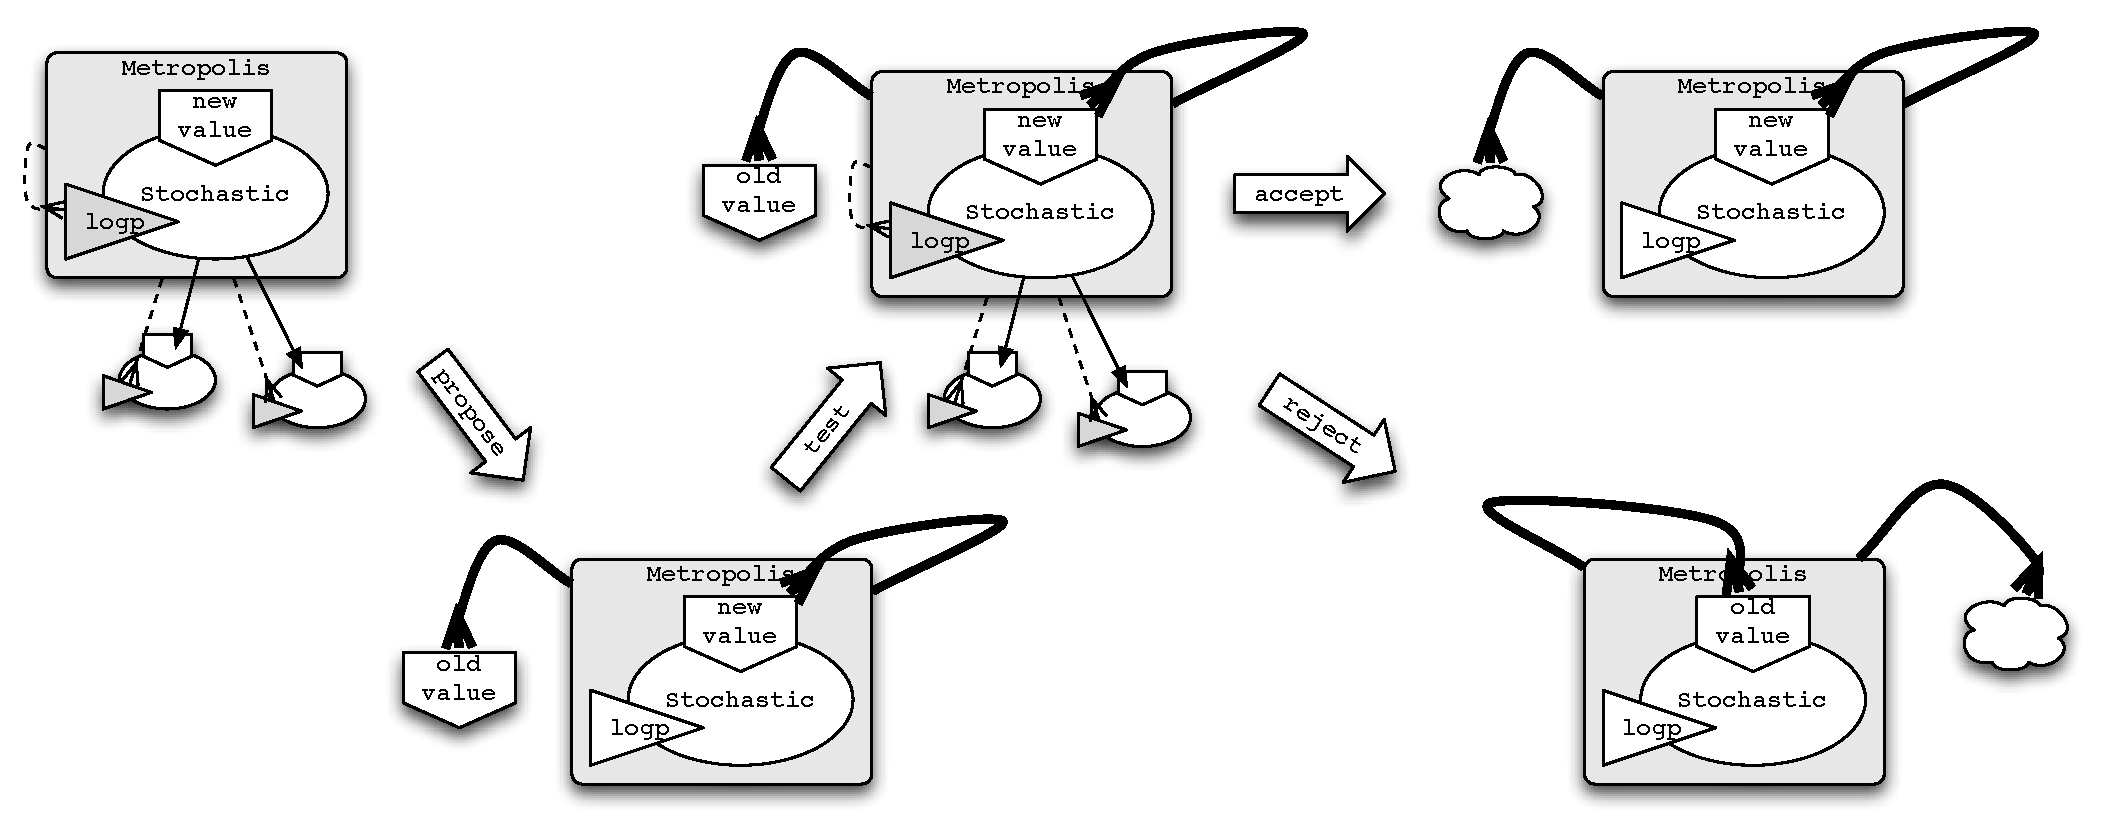
\epsfig{file=figs/sampmethod_cartoon.pdf,width=15cm}
    \caption{The action of a Metropolis step method when its \texttt{step} method is called. First, the variable's log-probability and the log-probabilities of its children are recorded and summed. Then, the variable's value is replaced with a proposed value. Then, the variable's log-probability and the log-probabilities of its children are queried and summed with the proposed value in place. If the jump is accepted, the old value is forgotten; if the jump is rejected, the proposed value is replaced with the old value and forgotten.}
    \label{metropoliscartoon}
\end{figure}

The simplest step method is the Metropolis step, implemented by class \texttt{Metropolis}. In addition to \texttt{step}, Metropolis step methods have a method called \texttt{propose} which assigns proposed values to the variables they handle and a method called \texttt{reject} which replaces the proposed values with the previous values. Suppose a Metropolis step method $S$ handles the random variable $B$. A call to $S$'s \texttt{step} method would result in the following chain of events, illustrated as a cartoon in figure \ref{metropoliscartoon}:
\begin{itemize}
    \item $B$'s log-probability is recorded.
    \item $B$'s log-likelihood (the sum of the log-probabilities of all $B$'s children) is recorded.
    \item $S$'s \texttt{propose} method is called.
    \begin{itemize}
        \item $B$'s value is set to a new value.
    \end{itemize}
    \item $B$'s log-probability and log-likelihood are computed.
    \item $B$'s proposed value is tested according to the Metropolis algorithm.
    \begin{itemize}
        \item If the test fails, $S$'s \texttt{reject} method is called.
        \begin{itemize}
            \item $B$'s value is reset to its last value.
            \item The method returns.
        \end{itemize}
        \item If the test passes, the method returns.
    \end{itemize}
\end{itemize}

\bigskip
Step methods can be created by the user. If the user fails to create a step method to handle a parameter, a default step method is assigned to the parameter as follows:
\begin{itemize}
    \item All available step method classes inspect the parameter and report their competences to handle it, on a scale of 0 to 1.
    \item An instance of the class reporting the highest competence is assigned to the parameter.
\end{itemize}

\section{GP realization-valued random variables}
\texttt{GP} objects are special random variables whose value attributes are \texttt{Realization} instances. A realization-valued parameter $f$ could be created as follows:
\begin{verbatim}
    f = GP(M, C, mesh=m)
\end{verbatim}
The third initialization argument \texttt{mesh} is an array of values, which will be incorporated into $f$ as the read-only attribute \texttt{mesh}.

Realization-valued parameters have log-probability attributes like any random variable, but of course it would usually be expensive and difficult to assign something like a log-density to an object representing an infinite-dimensional random variable. The log-probability attribute instead gives $p(f(m))|\texttt{M,C})$. In words, the log-probability attribute only returns the log-probabilty of $f$'s value's evaluation on its mesh.

\section{Step methods for realization-valued random variables and their parents}

The a price of the `cop-out' of computing realization-valued parameters' log-probabilities based only on their evaluation on a mesh is that the Metropolis-Hastings algorithm no longer applies. \texttt{GPMetropolis} and \texttt{GPParentMetropolis} employ a strategy that will be described here. Denote by $\tilde f$ the evaluation of $f$ everywhere except on $m$. Denote the parents of $f$ by $P$ and its `extended children', or the set of parameters descended from it either directly or via an unbroken sequence of deterministic variables, by $K$.

A very important point is that neither of the step methods in this section care at all about how $K$ depends on $f$. This means that, like the standard Metropolis algorithm in more mundane probability models, they can theoretically be applied in an enormous range of probability models that involve Gaussian processes. In practice, of course, novel step methods will often be desirable to speed convergence. I hope authors of such step methods will share their objects by making them available for distribution with Random Realizations.

\subsection{A Metropolis step method for realization-valued RV's} 
The Metropolis-Hastings acceptance ratio for a proposed value $f_p$ can be written as follows:
\begin{eqnarray*}
    \frac{p(K|\tilde f_p, f_p(m))\ p(f_p(m) | P)\ q(f(m)|f_p(m),P)}{p(K|\tilde f, f(m))\ p(f(m) | P)\ q(f_p(m)|f(m),P)} \frac{Q(\tilde f|f(m),P)}{Q(\tilde f_p|f_p(m), P)} ,
\end{eqnarray*}
where $q(f_p(m)|f(m),P)$ denotes the proposal density for $f(m)$ $Q(f|f(m), P)$ denotes the proposal density for $\tilde f$ with respect to $\tilde f$'s measure conditional on its parents and $f(m)$:
\begin{eqnarray*}
    Q(\tilde f|f(m),P) = \frac{d\theta(\tilde f|f(m),P)}{d\pi(\tilde f|f(m),P)},
\end{eqnarray*}
where the measures $\theta$ and $\pi$ denote the proposal and prior measures respectively. The troublesome terms involving $\tilde f$ and $\tilde f_p$ in the consequent position can be neglected if the proposal measure for $\tilde f$ is set to its measure conditional on its parents and $f(m)$, so that the density becomes 1; in other words, if $\tilde f$ is proposed from its prior conditional on $f(m)$. \texttt{GPMetropolis} step methods employ this strategy.

The evaluation $f(m)$ on the mesh is proposed from a multivariate normal distribution. By default, the covariance is a scalar multiple of $C(m,m)$, but this is tunable.

\subsection{Metropolis step methods for parents of realization-valued RV's} 
Similarly, the Metropolis-Hastings acceptance ratio for a proposed value $P_p$ of the parents \emph{and} a proposed value $\tilde f_p$ for the realization evaluated off the mesh is as follows:
\begin{eqnarray*}
    \frac{p(K|\tilde f_p)\ p(f(m) | P_p)\ q(P)}{p(K|\tilde f)\ p(f(m) | P)\ q(P_p)} \frac{Q(\tilde f|f(m),P)}{Q(\tilde f_p|f(m), P_p)}
\end{eqnarray*}
If the same proposal distribution as above is used for $\tilde f$, the intractable term again does not have to be computed. In other words, every time a value is proposed for one of $f$'s parents, a value is proposed for $f$ itself conditional on its evaluation on its mesh. 

To implement this strategy, \texttt{GPParentMetropolis} modifies a host \texttt{Metropolis} instance. It replaces its host step method's \texttt{propose} and \texttt{reject} methods with special methods that call the host's native methods, and then propose and reject values for $\tilde f$ conditional on $f(m)$. \texttt{GPParentMetropolis} also modifies the host step method to include the likelihood term $p(K|\tilde f)$ in the acceptance ratio.

This scheme works if $K$ depends on $P$ and if $P$ has extended children other than $f$, but for clarity these possibilites are not included in the acceptance ratio above. \texttt{GPParentMetropolis} can wrap Metropolis-Hastings step methods other than the simple Metropolis step method if desired.

\subsection{Choosing a mesh} If a GP-valued random variable is assigned an empty mesh $m$, its value will be proposed from its prior, and rejection rates are likely to be quite large. If the mesh is too dense, on the other hand, computation of the log-density will be expensive, as it scales as the cube of the number of points in the mesh. Several choices for mesh density and some corresponding proposals $\tilde f_p$ are shown in figure \ref{fig:meshpropose}. 

If the mesh is very dense, the Markov chain may occasionally explore values for the parameters of the covariance $C$ for which $C(m,m)$ is numerically singular. When \texttt{GPParentMetropolis} instances encounter this situation, they reject the jump and optionally display a warning. A more correct approach would be to simply thin the mesh and continue sampling, but I have not implemented this extension.

\begin{figure}
    \centering
        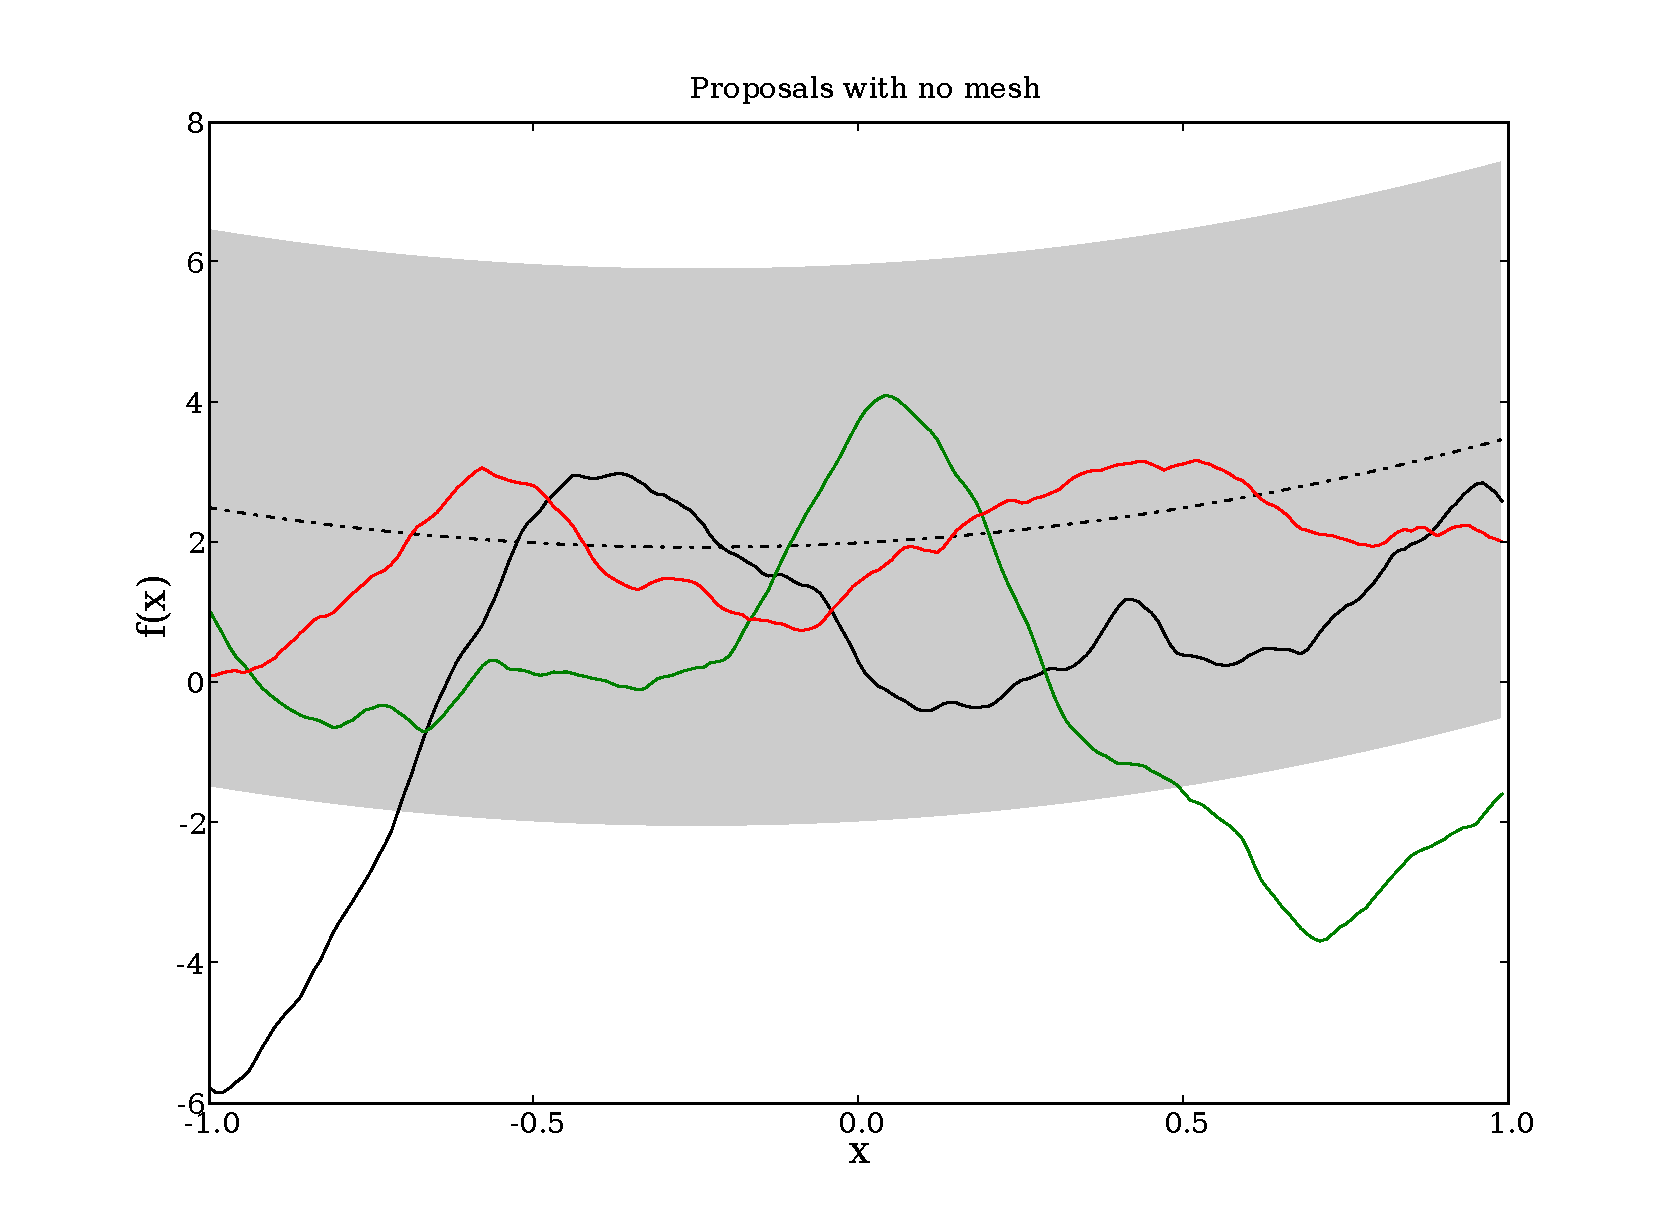
\epsfig{file=figs/nomeshpropose.pdf,width=8cm}
        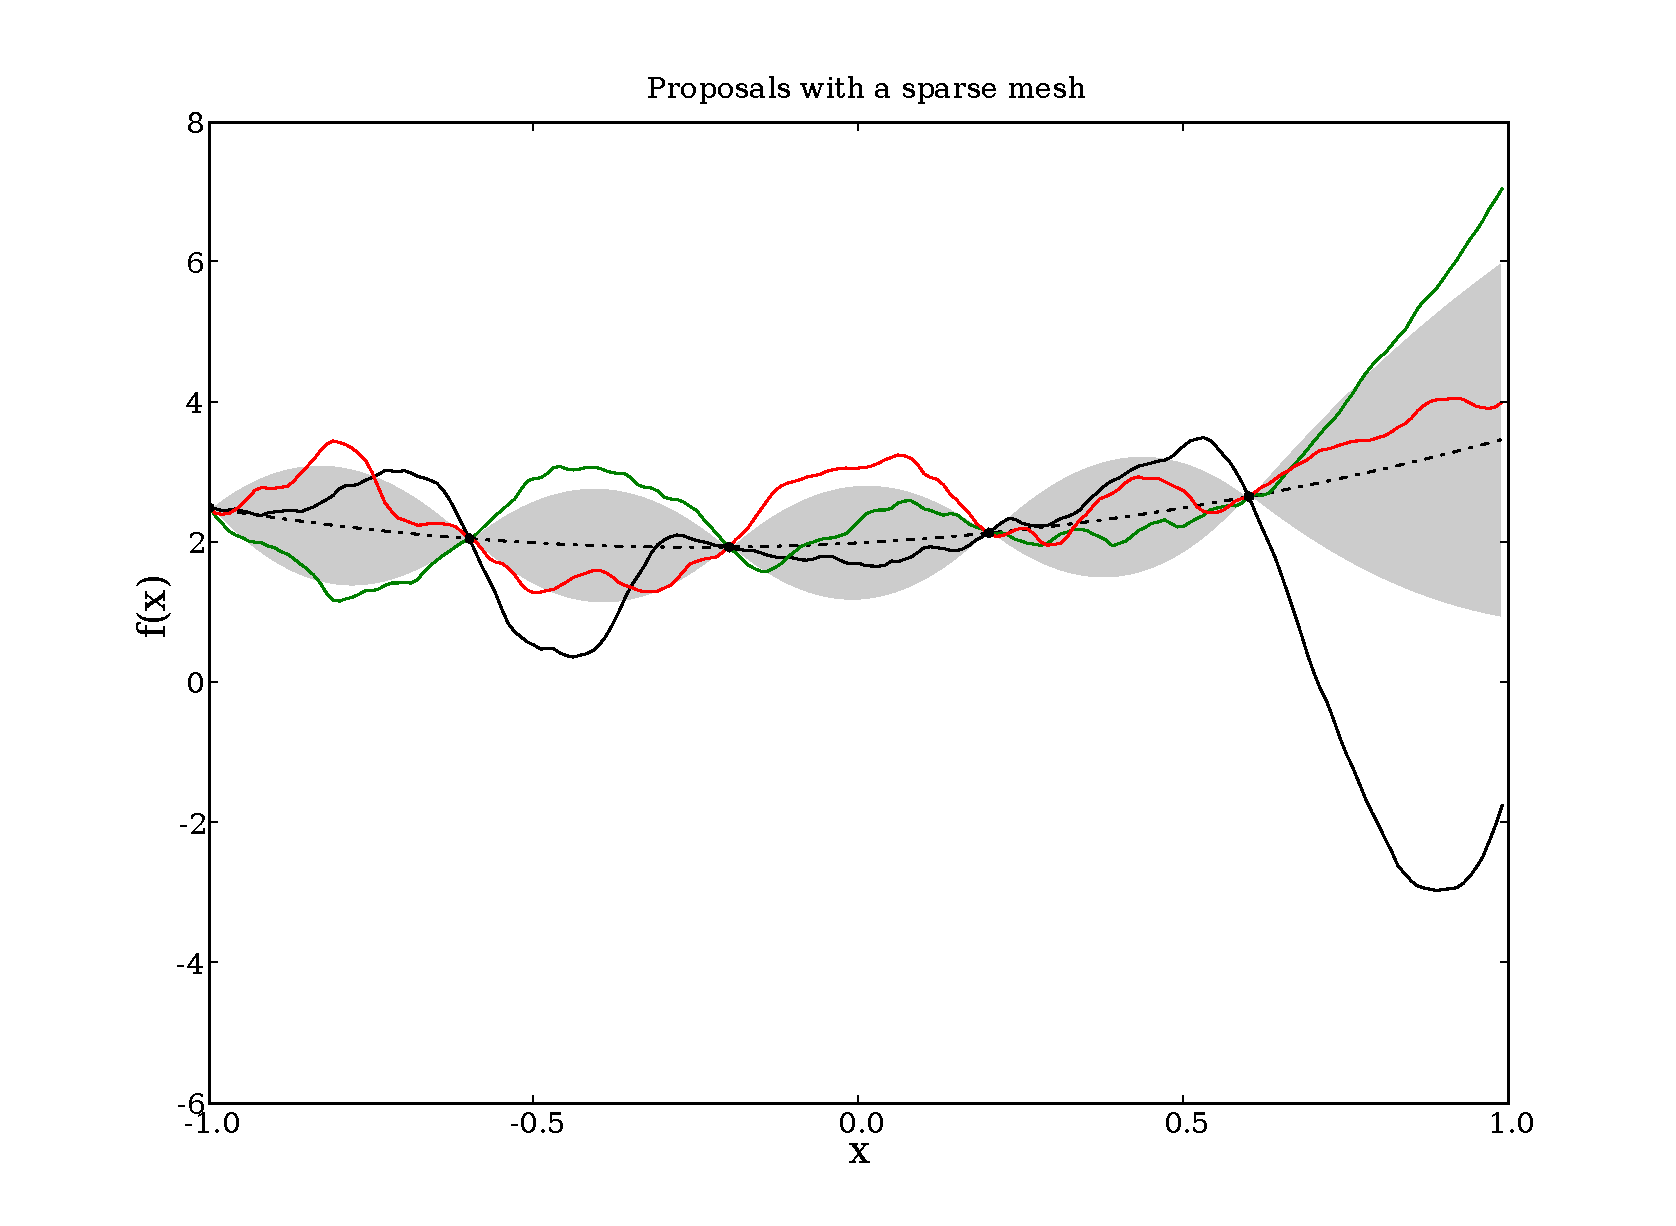
\epsfig{file=figs/lightmeshpropose.pdf,width=8cm}
        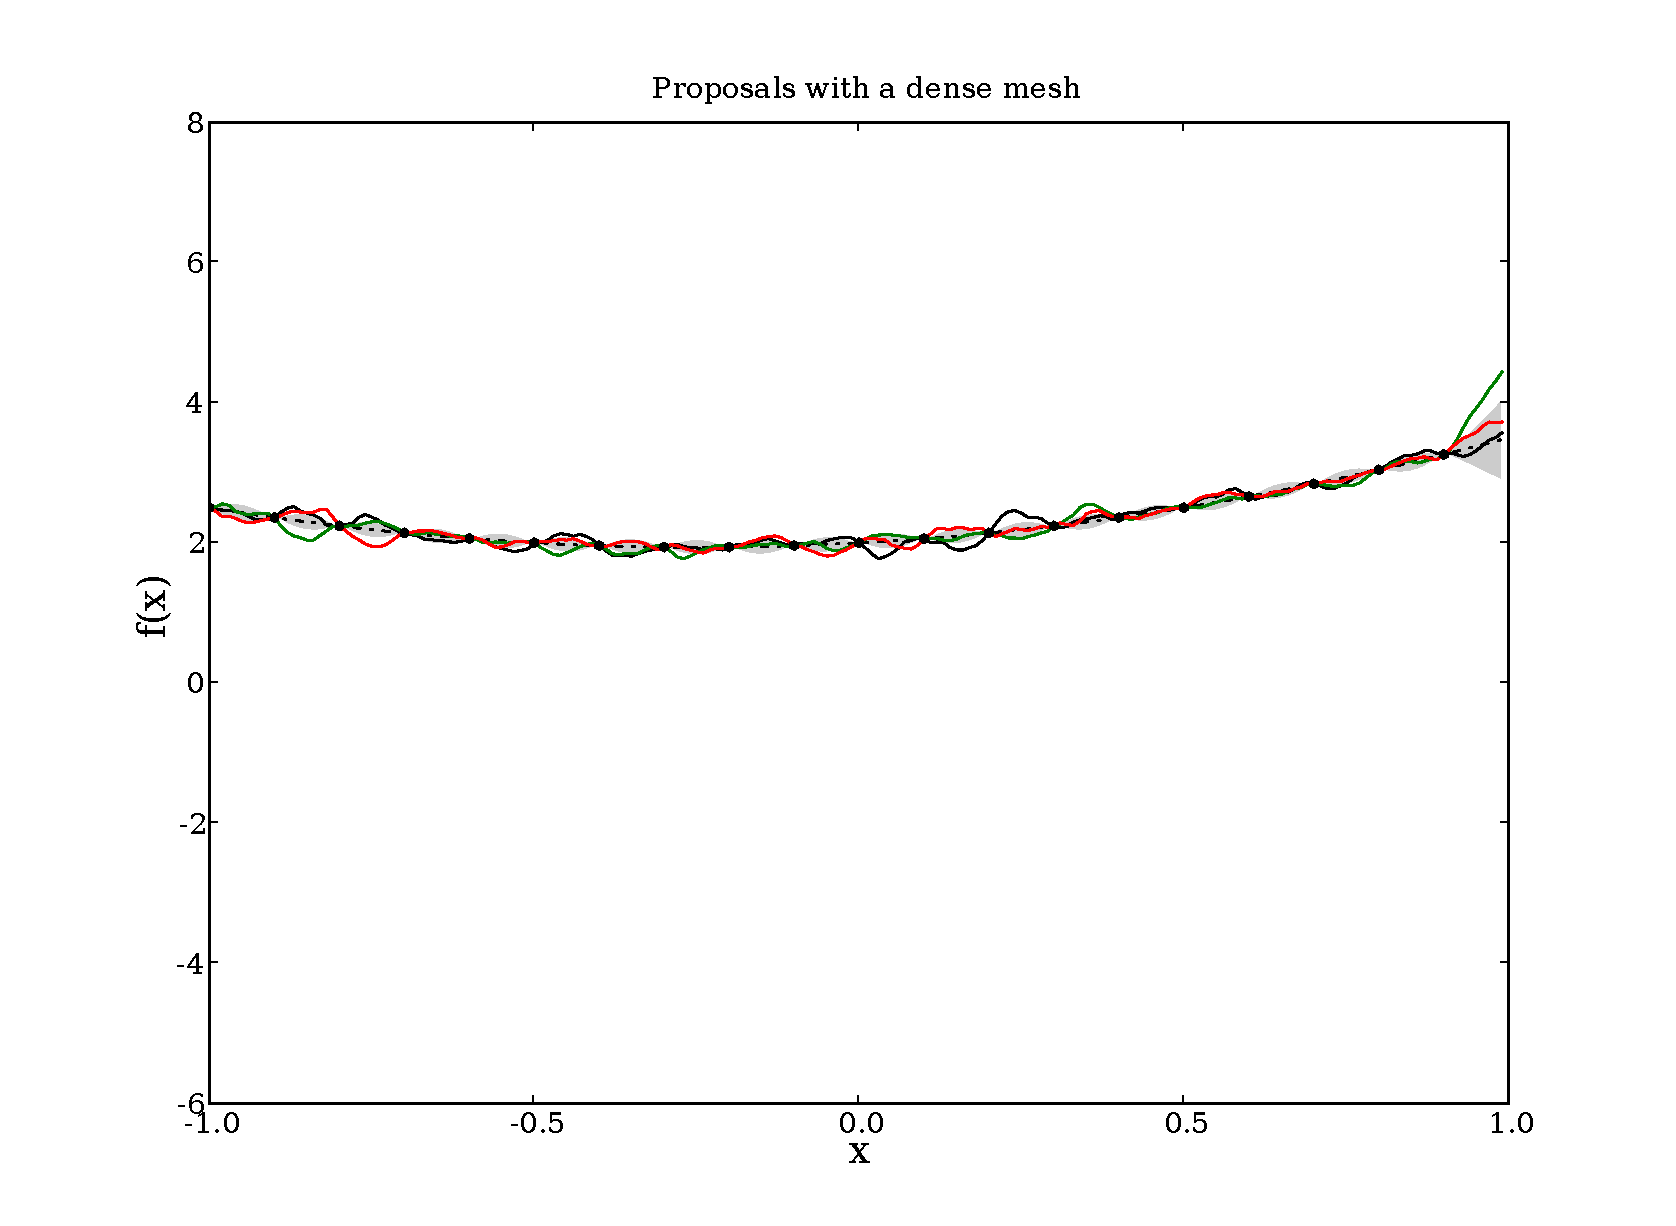
\epsfig{file=figs/densemeshpropose.pdf,width=8cm}        
    \caption{Several possible proposals of $\tilde f$ (curves) given proposed values for $f(m)$ (heavy dots) with no mesh (\textbf{top}), a sparse mesh (\textbf{middle}), and a dense mesh (\textbf{bottom}). Proposal distributions' one-standard-deviation envelopes are shown as shaded regions, with means shown as broken lines. With no mesh, $\tilde f$ is being proposed from its prior and the acceptance rate will be very low. A denser mesh permits a high degree of control over $\tilde f$, but computing the log-probability will be more expensive.}
    \label{fig:meshpropose}
\end{figure}


\section{Gibbs step methods for realization-valued random variables}
A realization-valued random variable's full conditional distribution \cite{gilks} is a Gaussian process if its Markov blanket \cite{jensen} is described by the following probability model:
\begin{eqnarray*}
    K_i |f \sim \textup{N}(f(o_i), V_i) & i=1\ldots N\\
    f|M,C\sim\textup{GP}(M,C)
\end{eqnarray*}
In other words, each of its children $K_i$ is normally distributed with variance $V_i$ and mean equal to $f(o_i)$, where each $o_i$ is an array of input values. In this case, $f$ can be handled by a \texttt{GPNormal} step method. These step methods maintain internal copies of $M$ and $C$, observed at input values $\{o_i\}$ with output values $\{K_i\}$ and variance $\{V_i\}$. 

An illustration of the respective performance of \texttt{GPMetropolis} and \texttt{GPNormal} for a model of the form
\begin{equation}
    \label{eqn:simple_GP_model}
    \begin{array}{l}
        d|f \sim \textup{N}(f(x),V)\\
        f|M,C\sim \textup{GP}(M,C)\\
        M|x= ax^2+bx+c\\
        C|x,y= \textup{Mat\`ern}(|x-y|,\nu, \phi, \alpha)\\
        \nu,\phi,\alpha,a,b,c,V\sim \textup{priors}          
    \end{array}
\end{equation}
with only two datapoints is shown in figure \ref{fig:MCMCOutput}. `Mat\`ern' indicates the Mat\`ern covariance function \cite{Banerjee}. 

\begin{figure}
    \centering
        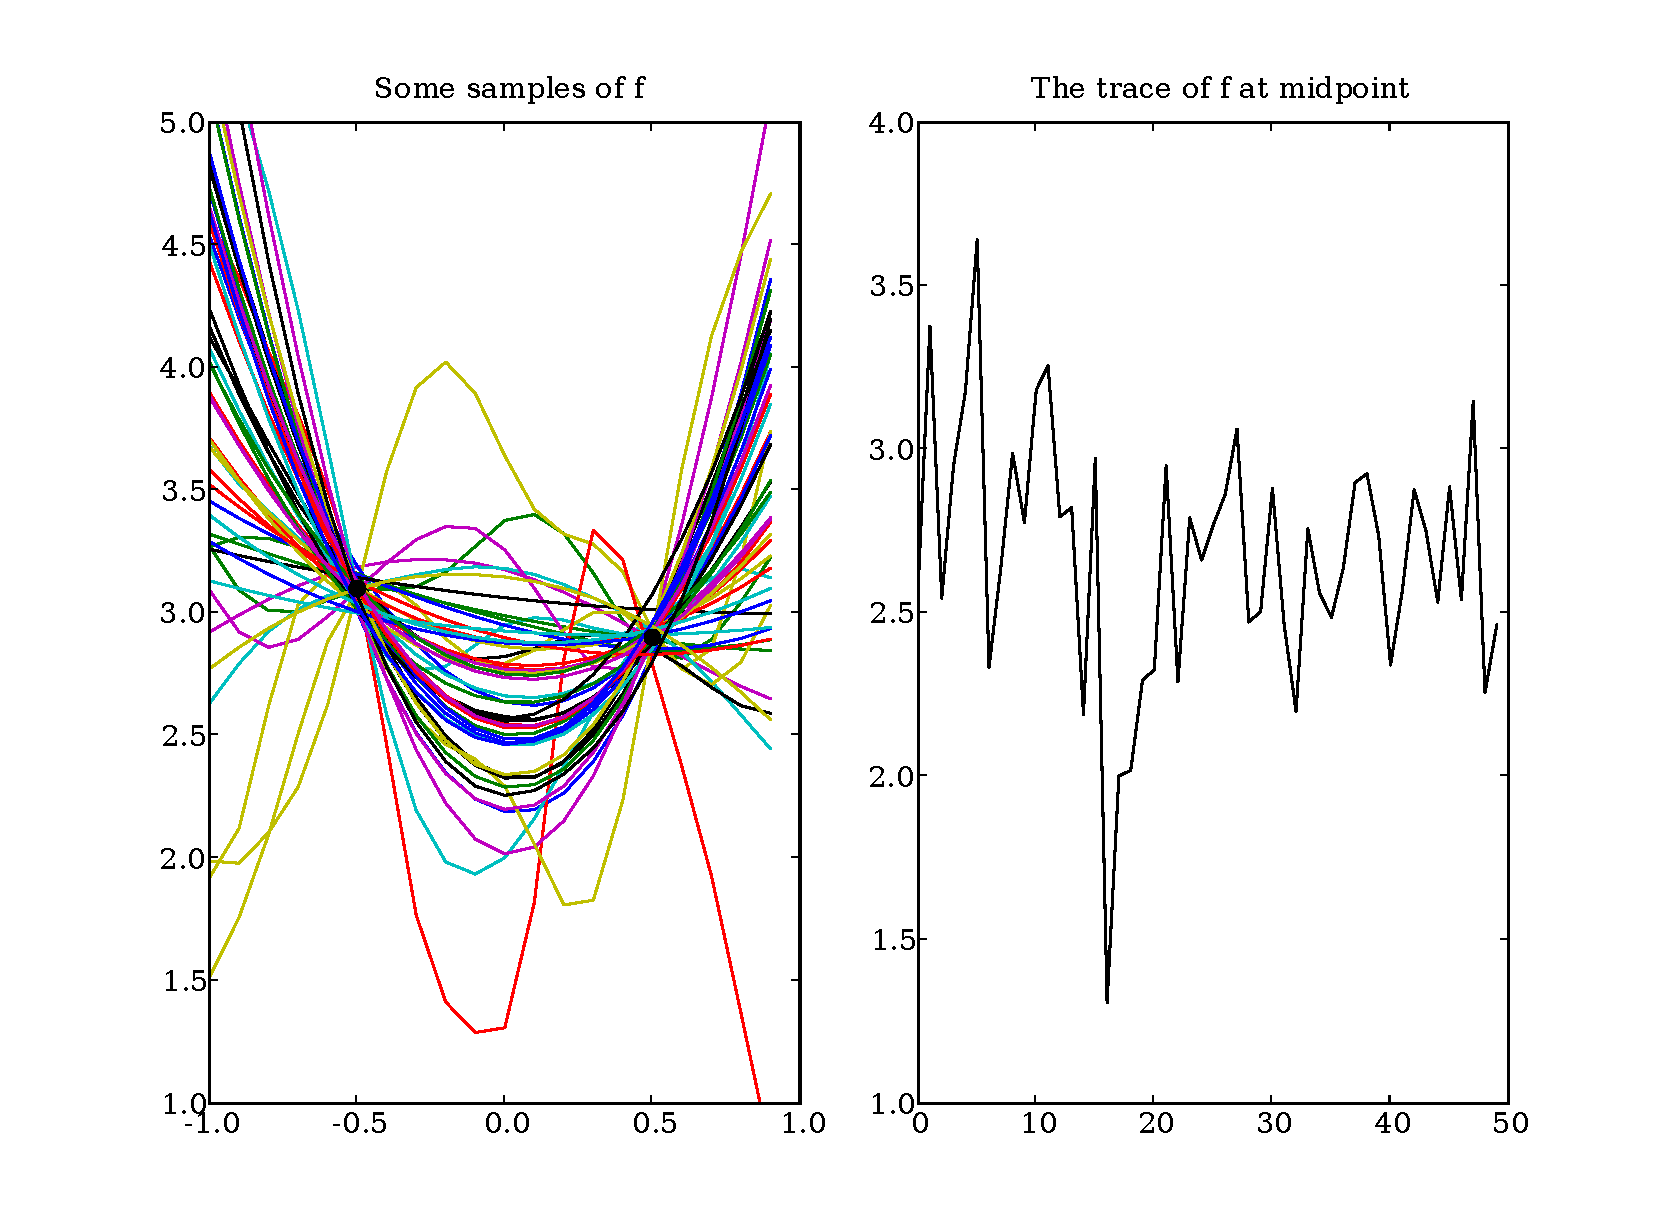
\epsfig{file=figs/gibbsSamples.pdf,width=12cm}
        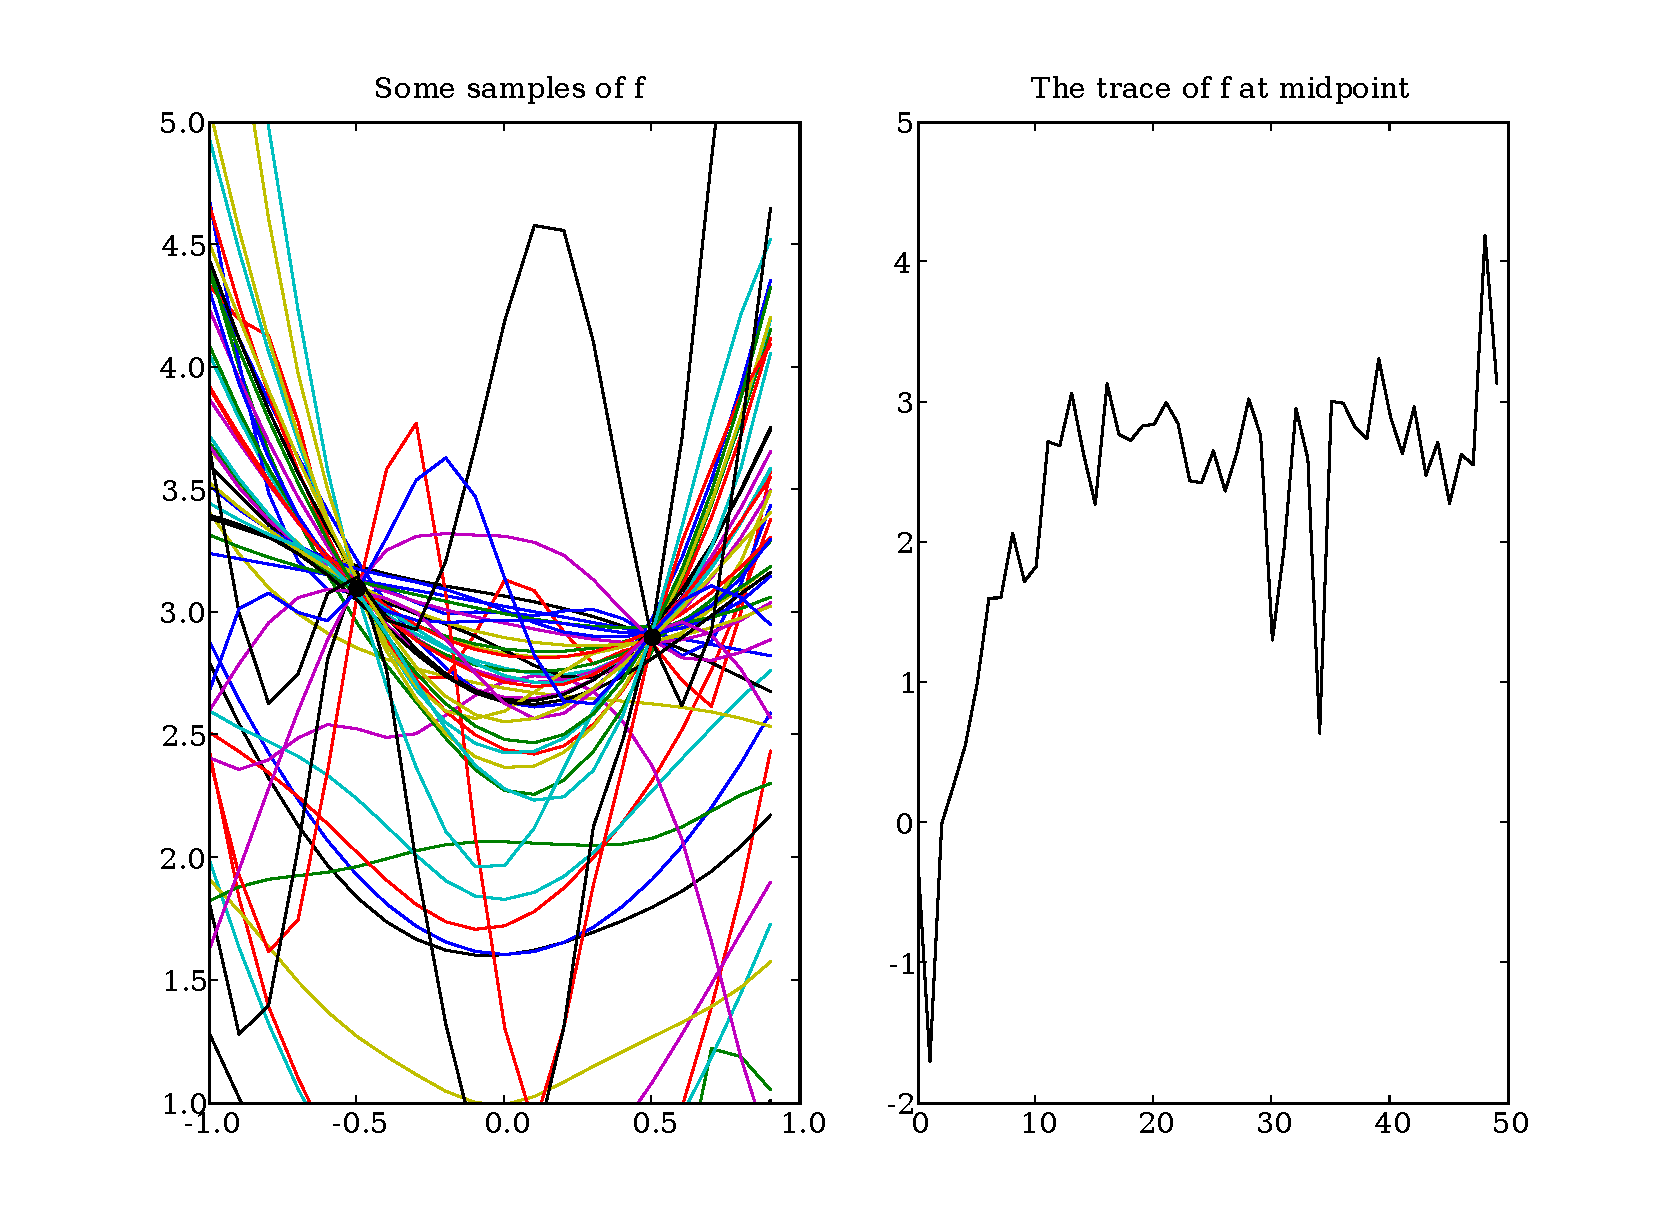
\epsfig{file=figs/metroSamples.pdf,width=12cm}          
    \caption{The output of an MCMC run for the model (\ref{eqn:simple_GP_model}) using the \texttt{GPNormal} (\textbf{top}) and \texttt{GPMetropolis} (\textbf{bottom}) step methods. Several samples are shown in the \textbf{left} panels, and the dynamic traces of the \texttt{GP}'s evaluation at the midpoint of the interval are shown in the \textbf{right} panels. Both the Metropolis and Gibbs samples' jumping distribution is modulated by the value of the prior parameters, which are updated by \texttt{GPParentMetropolis} step methods.}
    \label{fig:MCMCOutput}
\end{figure}

% \section{Example: Munch, Kottas and Mangel's stock-recruitment study}\label{sub:MMKMCMC}
% 
% As a less trivial example, consider Munch, Kottas and Mangel's \cite{Munch} inference of stock-recruitment functions from fishery science. Their probability model follows, with the minor modification that the Mat\`ern covariance function is used. Here $f$ is the stock-recruitment function, $C$ is its covariance and $M$ is its mean.
% \begin{equation}
%     \label{eqn:MMKModel}
%     \begin{array}{l}
%         \textup{frye}|f \sim \textup{N}(\exp(f(\log(\textup{abundance}))), V)\\
%         f\sim \textup{GP}(M,C)\\
%         M|x= \beta_0+\beta_1 \log(x)\\
%     C|x,y= \textup{Mat\`ern}(|x-y|,\nu, \phi, \alpha)\\        
%     V,\ \beta_0,\ \beta_1,\ \nu,\ \phi,\ \alpha \sim \textup{priors}.
%     \end{array}
% \end{equation} 
% The `priors' are provided by the authors (except the prior on $\nu$, which is described in the documentation \cite{me_SR} ). The posterior distribution of $f$ for pink salmon (\emph{Onchorhynchus gorbuscha}) is shown in figure \ref{fig:pinkfpost}. $f$ is handled by a \texttt{GPNormal} step method.
% 
% \begin{figure}
%     \centering
%         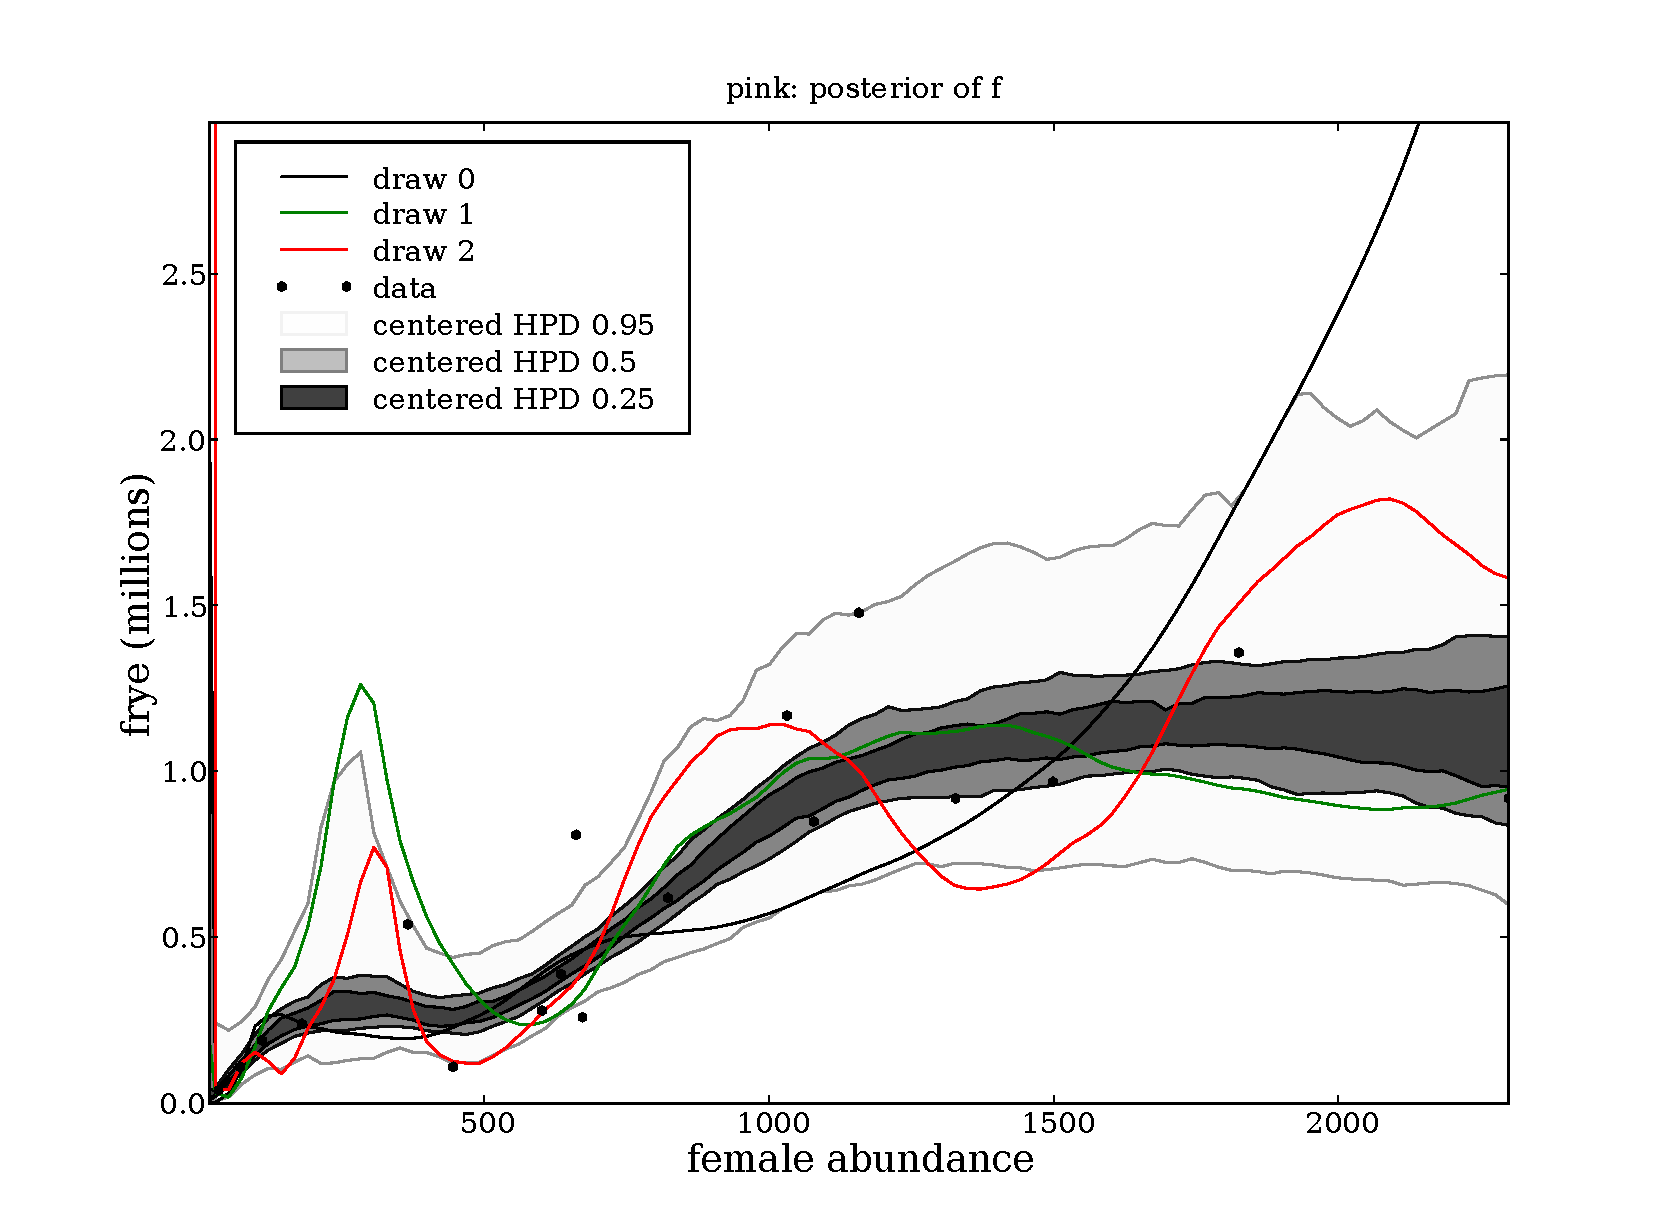
\epsfig{file=figs/pinkfpost.pdf, width=10cm}
%     \caption{The posterior of the stock-recruitment function for pink salmon (\emph{Onchorhynchus gorbuscha}). The data are shown as heavy black dots. The centered 95\%, 50\% and 25\% posterior probability intervals are shown as shaded regions. Three draws from the posterior are plotted.}
%     \label{fig:pinkfpost}
% \end{figure}

\chapter{Summary}
The following list of the objects with summaries of users' interaction with them:
\begin{itemize}
    \item \texttt{Mean} is a callable object, like a simple one-place function.
    \item \texttt{Covariance} is a callable object, like a simple two-place function. Its return value is a matrix. It can efficiently compute and return the Cholesky factorization or diagonal of that matrix instead, if desired.
    \item \texttt{Realization} is a callable object representing a draw from a Gaussian process. It can be created by typing \texttt{f = Realization(M, C)}. Once created, it behaves like a simple one-place function.
    \item \texttt{GP} is a random variable valued as a GP realization. It has a \texttt{value} attribute and a \texttt{logp} attribute, like an ordinary PyMC \texttt{Stochastic} object. An enormous variety of probability models involving Gaussian processes can be easily constructed using this object.
    \item \texttt{GPMetropolis}, \texttt{GPParentMetropolis} and \texttt{GPNormal} are step methods responsible for implementing Metropolis and Gibbs steps involving GP realization-valued parameters and their parents. Users often do not have to interact with the first two, because they are assigned and tuned automatically by PyMC.
\end{itemize}
\texttt{Mean} and \texttt{Covariance} can be modified by the function \texttt{observe}, which `imposes' normally-distributed observations on them.

The three basic objects, \texttt{Mean}, \texttt{Covariance} and \texttt{Realization}, resemble the concepts they represent very closely; as callable objects, they are as close to mathematical functions as programming language features can be. Because they can be created, manipulated and plotted in interactive Python sessions, I hope they prove to be of value as teaching and learning tools for building intuition about Gaussian processes without making lengthy excursions into linear algebra.

The other objects allow for Gaussian processes to be mixed into nearly arbitrary probability models. Using them, users can use the basic objects that have served them as models of Gaussian process-related concepts directly in statistics with ease comparable to that provided by WinBugs. The standard caveats of MCMC algorithms apply, of course; some models will be prohibitively expensive to fit, and some will have very poor mixing properties unless treated with specialized step methods. However, I hope that the decentralization and extensibility of PyMC's model-fitting approach eventually fosters the growth of a library of such step methods.

\bibliographystyle{plain}
\bibliography{Anand_Patil_Thesis}

\end{document} 